\documentclass{article}

\usepackage[backend=biber,sorting=none]{biblatex}
\addbibresource{mybib.bib}

\usepackage{amsmath}
\usepackage{graphicx}

\title{An Example Where Per-Token Coupling Does Not Optimally Couple Response Distributions}
\author{Malcolm Sharpe}
\date{\today}

\begin{document}

\maketitle

\begin{abstract}
Coupling LLM response distributions is useful for applications such as evaluation and speculative decoding. In standard speculative decoding, each token is optimally coupled, but residuals are sampled independently. We give a simple example where that coupling method does not optimally couple the response distributions.
\end{abstract}

\section*{Preliminaries}

\begin{itemize}
    \item \(X\) and \(Y\) are random variables drawn from the two response distributions.
    \item A coupling of \(X\) and \(Y\) introduces a dependency between \(X\) and \(Y\).
    \item Per-token-optimal coupling (PTOC) is the method for coupling response distributions implicit in standard speculative decoding \cite{leviathan2023fast} \cite{chen2023acceleratinglargelanguagemodel}. PTOC maximizes the probability that the current token is equal. Conditioned on the current token not being equal, the two current tokens are sampled independently.
    \item All-prefix-optimal coupling (APOC) is a method for coupling response distributions. APOC maximizes the probability that the two responses are equal.
\end{itemize}

\section*{Example}

Each response distribution is uniform:

\begin{align*}
    X &\sim \text{Uniform}(\{aa, ab, bb\}) \\
    Y &\sim \text{Uniform}(\{aa, ba, bb\})
\end{align*}

The optimal coupling of the responses (for example, obtained using APOC):

\[
(X, Y) \sim \text{Uniform}(\{(aa, aa), (ab, ba), (bb, bb)\})
\]

In that coupling, \(P[X = Y] = \frac{2}{3}\). PTOC however only achieves \(P[X = Y] = \frac{1}{3}\). (See Figure~\ref{fig:coupling_example}.)

\begin{figure}[ht]
    \centering
    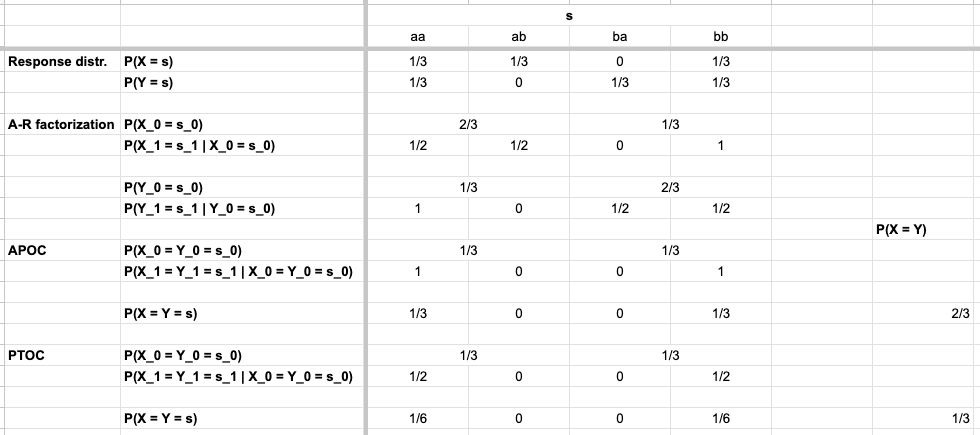
\includegraphics[width=\linewidth]{table1.png}
    \caption{The example response distributions, their auto-regressive factorizations, and their APOC and PTOC couplings.}
    \label{fig:coupling_example}
\end{figure}

\section*{Related Work}

Sun et al., in independent\footnote{The author blogged this example \cite{sharpe2024blogexample} and an early version of APOC \cite{sharpe2024blogapoc}.} work, presented APOC in the context of speculative decoding \cite{sun2024blockverificationacceleratesspeculative_v1}, as well as a different simple example for which PTOC does not optimally couple the response distributions \cite{sun2024blockverificationacceleratesspeculative_v2}.

\printbibliography

\end{document}
